\documentclass[12pt]{UoAthesis}
\usepackage{booktabs}
\thesistitle{Honours Dissertation}
\thesisauthor{Christopher James Thomson}
\thesispdfkeywords{}
\thesisyear{2012}

\thesisabstract{This is a short summary of my work...}
\acknowledgements{I would like to dedicate this work to..}

%%% The bibtex file where your references are stored
\bibliography{main}

\begin{document}

%%% = = = DISSERTATION OVERVIEW = = = %%%
% - Introduction - %
% - - Molecular dynamics, what is it, why is it important to Chemical
% - - engineering. Leading into potentials, need for faster methods,
% - - more accurate methods.
%
% Review of exisiting literature (Chapela, PRIME SPEADMD), what
% they've done, why its not as good as what you're going to do
%
% Outline of the thesis to come. 

% - Molecular Simulation 
% -- Newtonian mechanics F=MA, is it valid?
% -- Forces from potentials (conservative forces)
% Types of forces (gravitional (which is neglected)), pairwise forces
% leading to intermolecular potentials.

% --- Give an example soft potential (LJ), Introduce a discrete --
% -potential, hard sphere is the prototypical discrete potential, --
% -but there are stepped potentials too (Chapela). Talk about the --
% -advantages/disadvantages etc.

%%%% Lead out of the chapter with this
% --- Introduce discrete potentials, say they need a special method of solution (EDMD).
% - Simulation Methods - %
% - - Force Driven Simulators
% - - - Introduction and general algorithm 
% - - - Integrators: Euler, Verlet, Velocity Verlet, Gear...lit review to find more recent ones
% - - - Optimization: neighbour lists, truncation of the potential 
% - - - Adv/Disadv? or just within other relevant topics
% - - Event Driven Simulators
% - - - Introduction and general algorithm
% - - - Collision rules
% Actually older than force based, although not as popular.
% - - - Optimization: neighbour lists, O(1) priority queue algorithms, time warp algorithms
% - - Measuring System Properties
% - - - Radial Distribution Function
% - - - Temperature
% - - - Pressure
% - - - Coefficient of Diffusion
% - Results - %
% - 'Checking the simulators' - %
%   Direct comparision with Chapela
% - Discussion - %
% - Conclusions - %
% - Recommendations for future work - %
% - Appendices - %
% - - Derivation of collision rule for stepped potentials
%%% = = = END OVERVIEW = = = %%%

\chapter{Introduction}

Process simulation packages have become an integral part of chemical
engineering design.  Central to these simulation software is the
ability to predict the thermodynamic and transport properties of fluids.
%\printbibliography[heading=thesisChapterBib]

\chapter{Molecular Dynamics}
\section{Introduction}
The underlying assumption behind many molecular dynamics simulations
is that the particles move according to the laws of Newtonian
Mechanics.  The effects fo Quantum Mechanics are usually small unless
very light atoms (such as hydrogen or helium) are being simulated or
the particles are vibrating at very high rates \cite{Frenkel2002}

The fundamental identity of Newtonian Mechnanics is Newton's Second
Law of Motion \eqref{eq:Fma}. This equation allows the prediction of a
particle's trajectory provided that an initial position and velocity
is known; and the forces acting on that particle can be calculated for
any position or velocity.

\begin{equation}
  \vec{F} = m \vec{a} \label{eq:Fma}
\end{equation}

If a force depends only on the position of a particle it is known as a
conservative force.  Almost all forces considered in molecular
dynamics are of this type because atoms or molecules do not lose
energy due to friction or any other dissipative process.  

Conservative forces can be further subdivided into forces that depend
either on absolute position such as gravity or forces can depend on
position relative to another particle (intermolecular forces).
Gravity is usually neglected in MD simulations as the mass of atoms
and molecules is very small.

Only pairwise intermolecular forces are considered ie the total force
acting on a particle is the sum of the forces caused by every other
particle in the system \eqref{eq:pairwise}.

\begin{equation}
  \vec{F_i} = \sum_{j \not= i}^{}F_{i} \label{eq:pairwise}
\end{equation}

While the forces caused by groups of particles should also be
considered, this would severly complicate the simulation, and hence is
often ignored.

In MD simulations the intermolecular forces are usually described
using potentials.

\subsection{Potentials}
A potential is the function of potential energy with position, where
position is usually expressed as a set of orthogonal vectors such as
$x$, $y$ and $z$ in three dimensions. Conservative forces can be
calculated from their potential by equation
\ref{eq:forcePotential}. The gradient of the potential, denoted by
$\nabla$ is the partial differential of the potential in each
orthogonal direction.

\begin{equation}
  \vec{F}=-\nabla U \label{eq:forcePotential}
\end{equation}

A very popular potential used in molecular dynamics simulations is the
Lennard-Jones potential \cite{Lennard-Jones1924} (equation
\ref{eq:LJ}) as it is simple yet gives comparable results to
experimental values.

\begin{equation}
  U(r) = 4 \epsilon \left[ \left( \frac{\sigma}{r} \right)^{12} - \left( \frac{\sigma}{r} \right)^{6} \right] \label{eq:LJ}
\end{equation}

In equation \ref{eq:LJ}, $\epsilon$ is the depth of the energy well,
while $\sigma$ is the root of the Lennard-Jones potential which
corresponds to the change from attractive to repulsive forces (see
Lennard Jones Figures), this is taken to be the diameters of the
particles during the collision.
\begin{figure}
\begin{center}
\input{figures/ljPot}
\caption{Plot of the Lennard-Jones potential}
\label{fig:ljPot}
\end{center}
\end{figure}
%[Insert plots of the lennard jones energy and force]%
%[Insert massive potential from maginn possibly mention coulombs law, hertz's law?]%
\section{Force-Driven Simulators}
\subsection{Introduction}
Force-driven (or time driven) simulators are the most popular method
of simulating particles due to their relative simplicity and ability
to handle soft potentials.  Simulators of this kind were pioneered by
Rahman \cite{Rahman1964} who predicted physical properties of liquid
argon with reasonable accuracy.

The distinguishing feature between force-driven and event-driven
simulators is the way in which they move through time.  During
force-based simulations particles' positions and velocities are
calculated every unit of time, $\Delta t$ using the forces acting on
the particles.  These newly calculated values are then used to predict
the next set of particle positions.  This is then repeated over the
desired simulation time.

\subsection{Integrators}
Once the forces acting on a particle is known, that particle's
acceleration can be calculated using Newton's Second Law of Motion
(equation \ref{eq:Fmvdot}).

\begin{equation}
  \vec{F} =  m \frac{\partial^2 \vec{r}}{\partial t^2} \label{eq:Fmvdot}
\end{equation}

However, since acceleration is the second time derivative of position
(velocity is the first time deriviative), calculating the particle's
future position results in solving a differential equation of order 2
or higher since force, and hence acceleration likely changes with
time.  In order to accomplish this numerical integrators are used.

The majority of numerical integrators are based on Taylor Series
(equation \ref{eq:Taylor}).

\begin{equation}
  \vec{r}(t+\Delta t) = r(t) + \frac{\partial \vec{r}(t)}{\partial t}(\Delta t) + \frac{1}{2}\frac{\partial^2 \vec{r}(t)}{\partial t^2}\Delta t^2 + \frac{1}{3!}\frac{\partial^3 \vec{r}(t)}{\partial t^3}\Delta t^3 + \frac{1}{4!}\frac{\partial^4 \vec{r}(t)}{\partial t^4}\Delta t^4 + ... \label{eq:Taylor}
\end{equation}

The simplest integrator is Euler's Method which is just the Taylor
Series truncated after the acceleration term (equation
\ref{eq:Euler}).

\begin{equation}
  \vec{r}(t+\Delta t) = r(t) + \vec{v}(\Delta t) + \frac{1}{2}\vec{a}\Delta t^2 + \mathcal{O}(\Delta t^3) \label{eq:Euler}
\end{equation}

However this method suffers from large errors and is unstable
\cite{Haile1997} and is therefore rarely used. The Verlet Integrator
\cite{Verlet1967} improves upon Euler's method by combining the
forward timestep with a reverse timestep \eqref{eq:Verletpos}.  This
method is actually fourth order as the third (and first) derivative is
cancelled out during its derivation.  The Verlet integrator does not
include an equation to calculate the future velocity so the central
difference used by Verlet is often used \eqref{eq:VerletVel}.

\begin{subequations}
  \begin{align}
    \vec{r}(t + \Delta t) &= 2\vec{r}(t) - \vec{r}(t - \Delta t) + \vec{a}(t)\Delta t^2 + \mathcal{O}(\Delta t^4) \label{eq:Verletpos} \\
    \vec{v}(t+\Delta t) &= \frac{\vec{r}(t+\Delta t) - \vec{r}(t-\Delta t)}{2\Delta t} \label{eq:VerletVel}
  \end{align}
\end{subequations}

Integrators suffer from couple key failings that cause a systematic
gain of energy known as ``energy drift''. Firstly, integrators are
based on infinite Taylor series which cannot be fully implemented,
therefore they have to be truncated after a certain number of terms,
this introduces an error. Secondly, integrators struggle to predict
values of forces that have discontinuities in them, such as hard
spheres which only have forces on contact but not before, or
discontinuities introduced by truncating potentials to improve
simulator speed.  There are a couple of types of integrators that try
and reduce these problems.

Sympletic integrators have the useful property in that they, on
average, conserve energy \cite{Hairer2003}.  The most common
symplectic integrator used in MD is the Velocity Verlet Integrator
\cite{Swope1982} shown in \eqref{eq:VVerlet}.

\begin{subequations}
  \label{eq:VVerlet}
  \begin{align}
    \vec{r}(t + \Delta t) &= \vec{r}(t) + \vec{v}(t) \Delta t + \frac{1}{2}\vec{a}(t) \Delta t^2 + \mathcal{O}(\Delta t^4) \label{eq:VVerletpos} \\
    \vec{v}(t+\Delta t) &= \vec{v}(t) + \frac{\vec{a}(t)+\vec{a}(t+\Delta t)}{2}\Delta t \label{eq:VVerletVel} 
  \end{align}
\end{subequations}

The popularity of the Velocity Verlet is due to its computational
simplicity and its accuracy and stability at relatively long
timesteps.  It can even be expanded \cite{Khakimov2002} to maintain
its accuracy and stability at very long timesteps at a small extra
computational cost.  However the Velocity Verlet cannot be used in
systems that do not conserve energy, ie systems with dissipative
forces.

Another popular method of improving the traditional integrator is
predictor-corrector integrators.  These use a truncated Taylor series
to calculated a predicted value for the future position and higher
order time derivatives. The force is then calculated at this
predicited position, then the difference between the predicted
acceleration and the corrected acceleration calculated from the force
is used to correct the position and time derivatives.

The most popular predictor-corrector integrator is that of Gear
\cite{Gear1971}, using his 5th order algorithm. The predicted value for
the $i^{th}$ time derivative is shown in \eqref{eq:GearPredictor}, and
defining $\Delta \vec{a} = \vec{a}\,^{C} - \vec{a}\,^{P}$, the
corrected time derivatives can be calculated using
\eqref{eq:GearCorrector} with coefficients from \eqref{eq:GearCoeff}.

\begin{equation}
  \frac{\partial^{i}}{\partial t^{i}} \vec{r}\:^{P}(t+\Delta t) = \sum^{n}_{k=i} \frac{1}{k!}\frac{\partial^{i} }{\partial t^{i}} \vec{r}(t) \Delta t^{k} \label{eq:GearPredictor}
\end{equation}

\begin{equation}
  \frac{\partial^{i}}{\partial t^{i}} \vec{r}\:^{C}(t+\Delta t) = \frac{\partial^{i} }{\partial t^{i}} \vec{r}\:^{P}(t+\Delta t) +\frac{c_i}{\Delta t^i} \left(\frac{\Delta t^2}{2}\Delta \vec{a}\right)  \label{eq:GearCorrector}
\end{equation}
\begin{equation}
  c_0 = \frac{3}{16},\;\; c_1 = \frac{251}{360},\;\; c_2 = 1,\;\; c_3 = \frac{11}{18},\;\; c_4 = \frac{1}{6},\;\; c_5 = \frac{1}{60} \label{eq:GearCoeff}
\end{equation}

The Gear's algorithm, while more accurate at short timesteps than Verlet's integrator \cite{Haile1997}, suffers at long timesteps and is computationally more expensive.

\section{Event-Driven Simulators}
\subsection{Introduction}
Though force-driven simulators are more popular the first MD
simulation was done using an event-driven simulator by Alder and
Wainwright \cite{Alder1959}. Event-driven simulators move through time
by jumping between successive collisions.  These collisions last an
infinitesmall amount of time, and deliver an impulse between the
particles.  
\chapter{Methodology}
\section{Introduction}
The two simulators described in this chapter were coded in C++ using
the C++ Standard Library with the Boost [cite] library to handle
random number generation.
\section{Force-driven Simulator}
Force driven simuators are currently the dominant MD paradigm
therefore it was decided that the results from the stepped potentials
would be compared to the equivalent results obtained from a
force-driven simulator. In order to acquire these results a force-driven simulator was written.

The algorithm for the force driven simulator is as follows.
\begin{flushleft}
\begin{enumerate}
\item Initialisation
\item Calculate particles' future positions
\item Calculate the forces acting on the particles
\item Calculate the future velocities of particles
\item Run thermostat (if enabled)
\item Measure properties
\item Repeat steps 2-6 for the desired number of iterations
\end{enumerate}
\end{flushleft}

\subsection{Initialisation}
The particles are initialised in a Face Centered Cubic (FCC)
\nomenclature{A}{FCC}{Face Centered Cubic} structure.  The use of the
FCC lattice is common when simulating Lennard-Jones potentials as the
first force-driven simulation \cite{Rahman1964} was carried out using
liquid Argon which crystalises to a FCC lattice. 

Particle velocities are assigned randomly from a Gaussian distribution
with a mean, $\mu = 0$, and a standard deviation, $\sigma =
\sqrt{T^{*}}$, where $T^{*}$ is the desired reduced temperature.  The
velocities are then rescaled to ensure there net shift in linear
momentum in any direction by applying \eqref{eq:zeroLinearP} in each
orthongonal direction.

\begin{equation}
  v_{i}^{new} = v_{i}^{old} - \frac{1}{N} \sum^{N}_{i}v_{i}^{old} \label{eq:zeroLinearP}
\end{equation}

\subsection{Running Simulation}
The

\chapter{Results}
\section{Benchmarking}
\subsection{Introduction}
After a MD simulator has been created it is necessary to compare its
results with those generated by others, to verify that the simulator
works correctly. 
\subsection{Event-Driven Simulator}
The event-driven simulator was first tested running a hard sphere
simulation before testing the more complex stepped potentials.  A
single 'step' with a energy requirement sufficiently large such that
no particle could enter it.  The simulation was run once at a range of
densities using 864 particles at a reduced temperature of $T^*=1$ for
5 million collisions, the results were compared with those of Lue
\cite{Lue2005} in \ref{tab:benchhard}. The agreement between results
is good and lies within statistical uncertainty. The largest
discrepancies are in the values for the coefficient of diffusion at
low densities which is probably due to Lue's values were obtained
after 10 million collisions.

\begin{table}
  \caption{Comparison of results obtained by the event-driven
    simulator with literature values. $t_{avg}$ is the average time
    between collisions, $\langle\mathbf{\hat{r}} \cdot \Delta
    \mathbf{v} \rangle_{coll}$ is the average momentum transfer per
    collision, and D is the coefficient of diffusion.} \label{tab:benchhard}
  \begin{center}
    \begin{tabular}{l c c c c c c}
      \toprule 
      $\rho$ & \multicolumn{2}{c}{$t_{avg}$} &
      \multicolumn{2}{c}{$\langle\mathbf{\hat{r}} \cdot \Delta
        \mathbf{v} \rangle_{coll}$} & \multicolumn{2}{c}{D} \\
      \cmidrule(rl{0.75em}){2-3}
      \cmidrule(rl{0.75em}){4-5}
      \cmidrule(rl{0.75em}){6-7}
      & Simulator & Lue & Simulator & Lue & Simulator & Lue\\
      \midrule
      0.3 & 0.3052 & 0.3052 & 1.775 & 1.772 & 0.53 & 0.55 \\
      0.4 & 0.1944 & 0.1942 & 1.776 & 1.773 & 0.341 & 0.359 \\
      0.5 & 0.13024 & 0.13031 & 1.774 & 1.7724 & 0.247 & 0.247 \\
      0.6 & 0.08966 & 0.08968 & 1.771 & 1.7721 & 0.169 & 0.173 \\
      0.7 & 0.0625 & 0.0625 & 1.773 & 1.776 & 0.114 & 0.113 \\
      0.8 & 0.04365 & 0.0436 & 1.772 & 1.772 & 0.064 & 0.065 \\
      0.9 & 0.03029 & 0.03024 & 1.773 & 1.772 & 0.033 & 0.0327 \\
      \bottomrule
    \end{tabular}
  \end{center}
\end{table}

The simulator was then benchmarked using a step potential.  The
results were compared with Chapela et al \cite{Chapela1989} using
their 'Case 6' steps. The simulation was run for 1.5 million
collisions using 864 particles. Each simulation was run ten times and
the mean values and standard deviations are given in
\ref{tab:benchsoft}
\begin{table}
  \caption{Comparison of results obtained by the event-driven
    simulator with literature values using stepped potentials. Numbers
    in parenthesis indicate the uncertainty in the final
    digit. \label{tab:benchsoft}}
  \begin{center}
    \begin{tabular}{l c c c c c c}
      \toprule $\rho$ & \multicolumn{2}{c}{$\langle T\rangle$} &
      \multicolumn{2}{c}{$\langle U \rangle$} &
      \multicolumn{2}{c}{$\langle P \rangle$} \\
      \cmidrule(rl{0.75em}){2-3} 
      \cmidrule(rl{0.75em}){4-5}
      \cmidrule(rl{0.75em}){6-7} 
      & Simulator & Chapela et al & Simulator
      & Chapela et al & Simulator & Chapela et al\\
      \midrule 
      0.85 & 0.719(3) & 0.72 & -6.04(7) & -5.80 & -0.5(4) & 0.54 \\
      0.85 & 1.339(8) & 1.34 & -5.130(9) & -5.14 & 4.08(4) & 4.08 \\
      0.85 & 2.35(1) & 2.35 & -4.24(2) & -4.20 & 8.78(9) & 8.86 \\
      0.85 & 3.37(2) & 3.37 & -3.48(2) & -3.49 & 12.90(9) & 13.00 \\
      0.85 & 4.59(1) & 4.60 & -2.67(1) & -2.68 & 17.31(8) & 13.43 \\
      0.75 & 0.811(2) & 0.81 & -5.095(3) & -5.08 & -0.20(2) & -0.24 \\
      0.75 & 1.309(9) & 1.31 & -4.67(1) & -4.63 & 1.81(5) & 1.84 \\
      0.75 & 2.49(1) & 2.49 & -3.88(1) & -3.82 & 5.80(4) & 5.95 \\
      0.75 & 3.59(2) & 3.59 & -3.26(1) & -3.22 & 9.03(7) & 9.20 \\
      0.65 & 1.309(8) & 1.31 & -4.081(8) & -4.06 & 0.80(3) & 0.81 \\
      0.65 & 2.61(1) & 2.61 & -3.42(1) & -3.41 & 3.86(5) & 3.89 \\
      0.65 & 3.79(1) & 3.79 & -2.926(9) & -2.94 & 6.34(7) & 6.33  \\
      \bottomrule
    \end{tabular}
  \end{center}
\end{table}
%\section{Adding Figures}
%To add figures to your text, you need to use a series of commands, but
%you can just copy paste the one below and tweak it for your needs.
%\begin{figure}[htp]
%  \centering
%  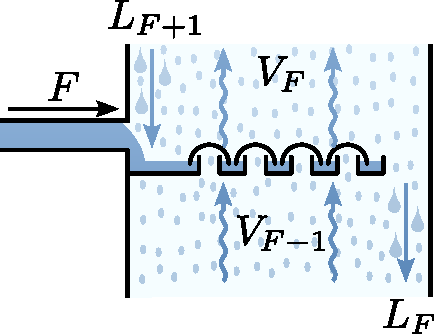
\includegraphics[clip,width=0.5\textwidth]{figures/testfig}
%  \caption{\label{fig:testfig} A test figure.}
%\end{figure}


%
%\section{References}
%You can reference entries in your bib file using the key you have set
%for it like so~\cite{Bannerman_2009}. I can even do cool things like
%say the author of that citation is \citeauthor{Bannerman_2009} and it
%was published in \citeyear{Bannerman_2009}. Or even ask for a full
%citation, like so: \fullcite{Bannerman_2009}.
%
%But you must remember to print the bibliography at the end of every
%chapter!
\newpage
\printbibliography[heading=thesisChapterBib]
\end{document}

%%%%TAYLOR SERIES FOR GEAR'S ALGORITHM%%%%
%\begin{equation}
%\begin{aligned}
%\vec{r}(t+\Delta t) &= \vec{r}(t) + \vec{v}(t) \Delta t 
%  + \frac{1}{2}\vec{a}(t)\Delta t^2 + \frac{1}{3!}\vec{b}(t)\Delta t^3
%  +  \frac{1}{4!}\vec{c}(t)\Delta t^4 + \frac{1}{5!}\vec{d}(t)\Delta t^5 \\
%\vec{v}(t+\Delta t) &= \vec{v}(t) \Delta t  + \vec{a}(t)\Delta t^2 
%  + \frac{1}{2}\vec{b}(t)\Delta t^3 + \frac{1}{3!}\vec{c}(t)\Delta t^4 + \frac{1}{4!}\vec{d}(t)\Delta t^5 \\
%\vec{a}(t+\Delta t) &= \vec{a}(t)\Delta t^2 + \vec{b}(t)\Delta t^3
%  +  \frac{1}{2!}\vec{c}(t)\Delta t^4 + \frac{1}{3!}\vec{d}(t)\Delta t^5 \\
%\vec{b}(t+\Delta t) &= \vec{b}(t)\Delta t^3 + \vec{c}(t)\Delta t^4 
%  + \frac{1}{2!}\vec{d}(t)\Delta t^5 \\
%\vec{c}(t+\Delta t) &= \vec{c}(t)\Delta t^4 + \vec{d}(t)\Delta t^5 \\
%\vec{d}(t+\Delta t) &= \vec{d}(t)\Delta t^5 \\
%\end{aligned}
%\end{equation}
